\documentclass{beamer}
\usepackage[utf8]{inputenc}
% \usepackage[latin1]{inputenc} %  Alternativ unter Windows
% \usepackage[T1]{fontenc}
\usepackage{dsfont}
\usepackage[ngerman]{babel}
\usepackage[toc,page]{appendix}
\usepackage{latexsym}
\usepackage{amsmath,amssymb,amsthm}
\usepackage{hyperref}

% einige Abkuerzungen, Funktionale fett mit eckigen Klammern, Mengen + Mengenfunktionen gestrichen, alle normalen Funktionen normale Klammern
\newcommand{\C}{\mathbb{C}} % komplexe
\newcommand{\K}{\mathbb{K}} % komplexe
\newcommand{\R}{\mathbb{R}} % reelle
\newcommand{\Q}{\mathbb{Q}} % rationale
\newcommand{\Z}{\mathbb{Z}} % ganze
\newcommand{\N}{\mathbb{N}} % natuerliche
\newcommand{\E}{\mathbf{E}} % Erwartungswert
\newcommand{\Var}{\mathbf{Var}} % Varianz
\newcommand{\Prob}{\mathbf{P}} % Wahrscheinlichkeit
\newcommand{\one}{\mathds{1}} % Charakteristische Funktion
\newcommand{\filtration}{\mathbb{F}} % Filtration
\newcommand{\F}{\mathcal{F}} %sigma-F
\newcommand{\id}{\text{id}} % Identität
\newcommand{\Zet}{Z}
\newcommand{\z}{\mathbf{z}}
\newcommand{\s}{\mathbf{s}}
\newcommand{\te}{\mathbf{t}}
\renewcommand{\P}{\mathbf{P}}
\renewcommand{\Q}{\mathbf{Q}}
\newcommand{\p}{\mathbf{p}}
\newcommand{\q}{\mathbf{q}}
\newcommand{\supp}{\text{supp}}

\newtheorem{Algorithmus}{Algorithmus}
\useoutertheme{infolines}
\beamertemplatenavigationsymbolsempty
\setbeamertemplate{headline}{}

\newcommand{\CoEx}[2]{\E\left[\left. #1\,\right| #2\right]}

\title{Seminar Statistische Lernverfahren}
\subtitle{Klassifikation von Rezensionstypen}
\author[T.G., A.K., M.L., T.N., M.H., J.S.]{Till Gräfenberg, Alexander Kohlscheen, Michael Lau, Tanja Niklas, Matthias Häußler, Jonathan Schmitz}
\date{12. Dezember 2019}
\begin{document}
\begin{frame}
\thispagestyle{empty}
\titlepage
\end{frame}

%<-------------Folie--------->
\section{Analysemethoden}
\begin{frame}
\frametitle{Analysemethoden}
\framesubtitle{Entscheidungsbaum}
\begin{itemize}\setlength\parskip{12pt}
\item Teilt in Klassen auf
\item Wahr oder Falsch Entscheidungen
\item Jedes Blatt hat genau eine Klasse
\item Verwende \texttt{rpart}
\end{itemize}
\begin{center}
	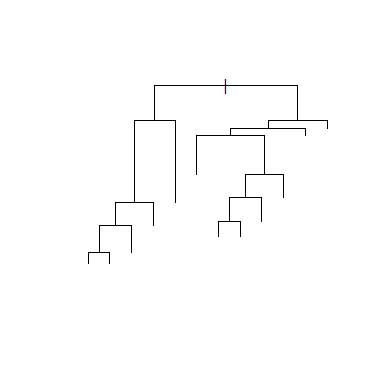
\includegraphics[scale=0.5]{RPart.png}
\end{center}
\end{frame}
%<-------------Folie--------->
\begin{frame}
\frametitle{Resultate Entscheidungsbaum, R, mind. 20 mal Wörter}
\begin{center}
\begin{tabular}{r|c|c|c|c|}
 &  Dominant  & Gewissenhaft & Initiativ & Stetig\\
\hline
Dominant & 14 & 3 & 9 & 1 \\
Gewissenhaft & 0 & 3 & 5 & 5\\
Initiativ & 2 & 4 & 19 & 5\\
Stetig & 2 & 4 & 3 & 7
\end{tabular}
\end{center}
\end{frame}
%<-------------Folie--------->
\begin{frame}
\frametitle{Resultate Entscheidungsbaum, R, mind. 20 mal Wörter}
\begin{center}
\begin{tabular}{r|c|c|c|}
 &  Precision  & Recall & F1 \\
\hline
Dominant     & 51,8\% & 77,7\% & 62,1\% \\
Gewissenhaft & 23,0\% & 21,4\% & 22,1\% \\
Initiativ    & 63,3\% & 52,7\% & 57,5\% \\
Stetig       & 43,7\% & 38,8\% & 41,1\% \\
\hline
Macro        & 45,4\% & 47,6\% & 45,4\%
\end{tabular}
\end{center}
\end{frame}
%<-------------Folie--------->
\begin{frame}
\frametitle{Resultate Entscheidungsbaum, Python, mind. in 1\% der Texte, englisch}
\begin{center}
\begin{tabular}{r|c|c|c|c|}
 &  Dominant  & Gewissenhaft & Initiativ & Stetig\\
\hline
Dominant &     9 & 4 & 12 & 5 \\
Gewissenhaft & 2 & 3 & 4 & 2\\
Initiativ &    5 & 5 & 12 & 8\\
Stetig &       2 & 2 & 8 & 3
\end{tabular}
\end{center}
\end{frame}
%<-------------Folie--------->
\begin{frame}
\frametitle{Resultate Entscheidungsbaum, Python, mind. in 1\% der Texte, englisch}
\begin{center}
\begin{tabular}{r|c|c|c|}
 &  Precision  & Recall & F1 \\
\hline
Dominant     & 30,0\% & 50,0\% & 37,5\% \\
Gewissenhaft & 27,2\% & 21,4\% & 23,9\% \\
Initiativ    & 40,0\% & 33,3\% & 36,3\% \\
Stetig       & 20,0\% & 16,6\% & 18,1\% \\
\hline
Macro        & 29,3\% & 30,3\% & 28,9\%
\end{tabular}
\end{center}
\end{frame}
%<-------------Folie--------->
\begin{frame}
\frametitle{Resultate Entscheidungsbaum, Python, mind. in 1\% der Texte, deutsch}
\begin{center}
\begin{tabular}{r|c|c|c|c|}
 &  Dominant  & Gewissenhaft & Initiativ & Stetig\\
\hline
Dominant &     13 & 4 & 16 & 1 \\
Gewissenhaft & 2 & 4 & 1 & 3\\
Initiativ &    3 & 5 & 13 & 7\\
Stetig &       0 & 1 & 6 & 7
\end{tabular}
\end{center}
\end{frame}
%<-------------Folie--------->
\begin{frame}
\frametitle{Resultate Entscheidungsbaum, Python, mind. in 1\% der Texte, deutsch}
\begin{center}
\begin{tabular}{r|c|c|c|}
 &  Precision  & Recall & F1 \\
\hline
Dominant     & 38,2\% & 72,2\% & 49,9\% \\
Gewissenhaft & 40,0\% & 28,5\% & 33,2\% \\
Initiativ    & 46,4\% & 36,1\% & 40,6\% \\
Stetig       & 50,0\% & 38,8\% & 43,6\% \\
\hline
Macro        & 43,6\% & 43,9\% & 41,8\%
\end{tabular}
\end{center}
\end{frame}
%<-------------Folie--------->
\begin{frame}
\frametitle{Analysemethoden}
\framesubtitle{Random Forest}
\begin{itemize}\setlength\parskip{12pt}
\item Entscheidungsbaum nicht beste Option
\begin{itemize}
	\item gut für Trainingsdaten
	\item nicht flexibel 
	\item Probleme mit neuen Datensätzen
\end{itemize}
\item Generiere neue Testdaten durch Wählen mit Zurücklegen
\item Erzeuge Entscheidungsbaum
\item Generiere so viele Entscheidungsbäume
\item Entscheidung durch Mehrheitsentscheidung
\item \texttt{R} \texttt{randomForest} 2000 Bäume
\end{itemize}
\end{frame}
%<-------------Folie--------->
\begin{frame}
\frametitle{Resultate Random Forest, R, mind. 20 mal Wörter}
\begin{center}
\begin{tabular}{r|c|c|c|c|}
 &  Dominant  & Gewissenhaft & Initiativ & Stetig\\
\hline
Dominant & 14 & 2 & 10& 0 \\
Gewissenhaft & 2 & 4 & 0 & 1\\
Initiativ & 2 & 7  & 25 & 14\\
Stetig & 0 & 1 & 1 &  3
\end{tabular}
\end{center}
\end{frame}
%<-------------Folie--------->
\begin{frame}
\frametitle{Resultate Random Forst, R, mind. 20 mal Wörter}
\begin{center}
\begin{tabular}{r|c|c|c|}
 &  Precision  & Recall & F1 \\
\hline
Dominant     & 53,8\% & 77,7\% & 63,5\% \\
Gewissenhaft & 57,1\% & 28,5\% & 28,0\% \\
Initiativ    & 52,0\% & 69,4\% & 59,4\% \\
Stetig       & 60,0\% & 16,6\% & 26,0\% \\
\hline
Macro        & 55,7\% & 48,0\% & 44,2\%
\end{tabular}
\end{center}
\end{frame}
%<-------------Folie--------->
\begin{frame}
\frametitle{Resultate Random Forest, Python, mind. in 1\% der Texte, englisch}
\begin{center}
\begin{tabular}{r|c|c|c|c|}
 &  Dominant  & Gewissenhaft & Initiativ & Stetig\\
\hline
Dominant & 16 & 4 & 14 & 4 \\
Gewissenhaft & 0 & 6 & 2 & 1\\
Initiativ & 1 & 4 & 16 & 9\\
Stetig & 1 & 0 & 4 & 4
\end{tabular}
\end{center}
\end{frame}
%<-------------Folie--------->
\begin{frame}
\frametitle{Resultate Random Forest, Python, mind. in 1\% der Texte, englisch}
\begin{center}
\begin{tabular}{r|c|c|c|}
 &  Precision  & Recall & F1 \\
\hline
Dominant     & 42,1\% & 88,8\% & 57,1\% \\
Gewissenhaft & 66,6\% & 42,8\% & 52,1\% \\
Initiativ    & 53,3\% & 44,4\% & 48,4\% \\
Stetig       & 44,4\% & 22,2\% & 29,6\% \\
\hline
Macro        & 51,6\% & 49,5\% & 46,8\%
\end{tabular}
\end{center}
\end{frame}
%<-------------Folie--------->
\begin{frame}
\frametitle{Resultate Random Forest, Python, mind. in 1\% der Texte, deutsch}
\begin{center}
\begin{tabular}{r|c|c|c|c|}
 &  Dominant  & Gewissenhaft & Initiativ & Stetig\\
\hline
Dominant & 15 & 4 & 15 & 2 \\
Gewissenhaft & 0 & 3 & 4 & 3\\
Initiativ & 2 & 4 & 15 & 9\\
Stetig & 1 & 3 & 2 & 4
\end{tabular}
\end{center}
\end{frame}
%<-------------Folie--------->
\begin{frame}
\frametitle{Resultate Random Forest, Python, mind. in 1\% der Texte, deutsch}
\begin{center}
\begin{tabular}{r|c|c|c|}
 &  Precision  & Recall & F1 \\
\hline
Dominant     & 41,6\% & 83,3\% & 55,4\% \\
Gewissenhaft & 30,0\% & 21,4\% & 24,9\% \\
Initiativ    & 50,0\% & 41,6\% & 45,4\% \\
Stetig       & 40,0\% & 22,2\% & 28,5\% \\
\hline
Macro        & 40,4\% & 42,1\% & 38,5\%
\end{tabular}
\end{center}
\end{frame}
\end{document}